\documentclass{beamer}

%--------------------
% Preámbulo
%--------------------

\mode<presentation> {
	\usetheme{default}
	\usecolortheme{beaver}
}	

\usepackage{adjustbox}
\usepackage{amsmath}
\usepackage{apacite}
\usepackage{booktabs}	
\usepackage{graphicx}
\graphicspath{ {figuras/} }
\usepackage{makecell}
\usepackage[round]{natbib}
\usepackage{sansmathaccent}
	\pdfmapfile{+sansmathaccent.map}
% Hyperref
\usepackage{hyperref}
\hypersetup{
	colorlinks=true,
	citecolor=red,
	filecolor=red,
	linkcolor=red,      
	urlcolor=blue,
}

% Aumentar espacio entre bullets
\let\tempone\itemize
\let\temptwo\enditemize
\renewenvironment{itemize}{\tempone\addtolength{\itemsep}{0.5\baselineskip}}{\temptwo}

%--------------------
% Título
%--------------------

\title[Actividad Tema I]{
	Actividad Tema I
}

\author{Desarrollo y Bienestar}
\institute[Iecon-FCEA-UdelaR]{
	Facultad de Ciencias Económicas y de Administración \\
	\medskip
	Universidad de la República
}

\date{29/08/2019}

%--------------------
%% Comienzo documento
%--------------------

\begin{document}
	
	%--------------------
	%% Título
	%--------------------	
	
	\begin{frame}
		\titlepage
	\end{frame}

	%--------------------
	%% Título
	%--------------------	
	
	\begin{frame}{Repaso}
	\textbf{Historia del palo de hockey}
	\bigskip
	\begin{itemize}
		\item Revolución industrial $\Leftrightarrow$ Revolución capitalista 
		\item Comienza en Gran Bretaña a mediados del siglo XVIII
		\item \textbf{Revolución industrial}
		\begin{itemize}
			\item revolución tecnológica permanente
		\end{itemize}
		\item \textbf{Revolución capitalista}
		\begin{itemize}
			\item capitalismo $\Rightarrow$ sistema económico $\Rightarrow$ instituciones
			\item ¿Qué instituciones?
			\begin{itemize}
				\item propiedad privada
				\item mercados
				\item empresas
			\end{itemize}
		\end{itemize}
	\end{itemize}
	\end{frame}

	\begin{frame}{Capitalismo}
		\textbf{¿Todos los sistemas capitalistas funcionan igual?} \\~\\ 
		\pause
		Dos tipos de condiciones contribuyen al dinamismo de un sistema capitalista:
		\pause
		\medskip
		\begin{itemize}
			\item condiciones económicas
			\begin{itemize}
				\item seguridad sobre la propiedad privada
				\item mercados competitivos
			\end{itemize}
			\item condiciones políticas
			\begin{itemize}
				\item garantizan las condiciones económicas
				\item proveen bienes y servicios no producidos por el mercado
			\end{itemize} 
		\end{itemize}
	\end{frame}

	\begin{frame}{Objetivo}
		En esta actividad intentaremos aplicar lo aprendido hasta ahora para dar respuesta a las siguientes preguntas:
		\bigskip
		\begin{enumerate}
			\item ¿Qué explica el crecimiento sostenido de China en las últimas décadas?
			\medskip
			\item ¿Puede ser este tipo de crecimiento sostenible? ¿Se trata de un sistema dinámico?
		\end{enumerate}		
	\end{frame}

	\begin{frame}{Creciendo como China}
		\begin{figure}
			\centering
			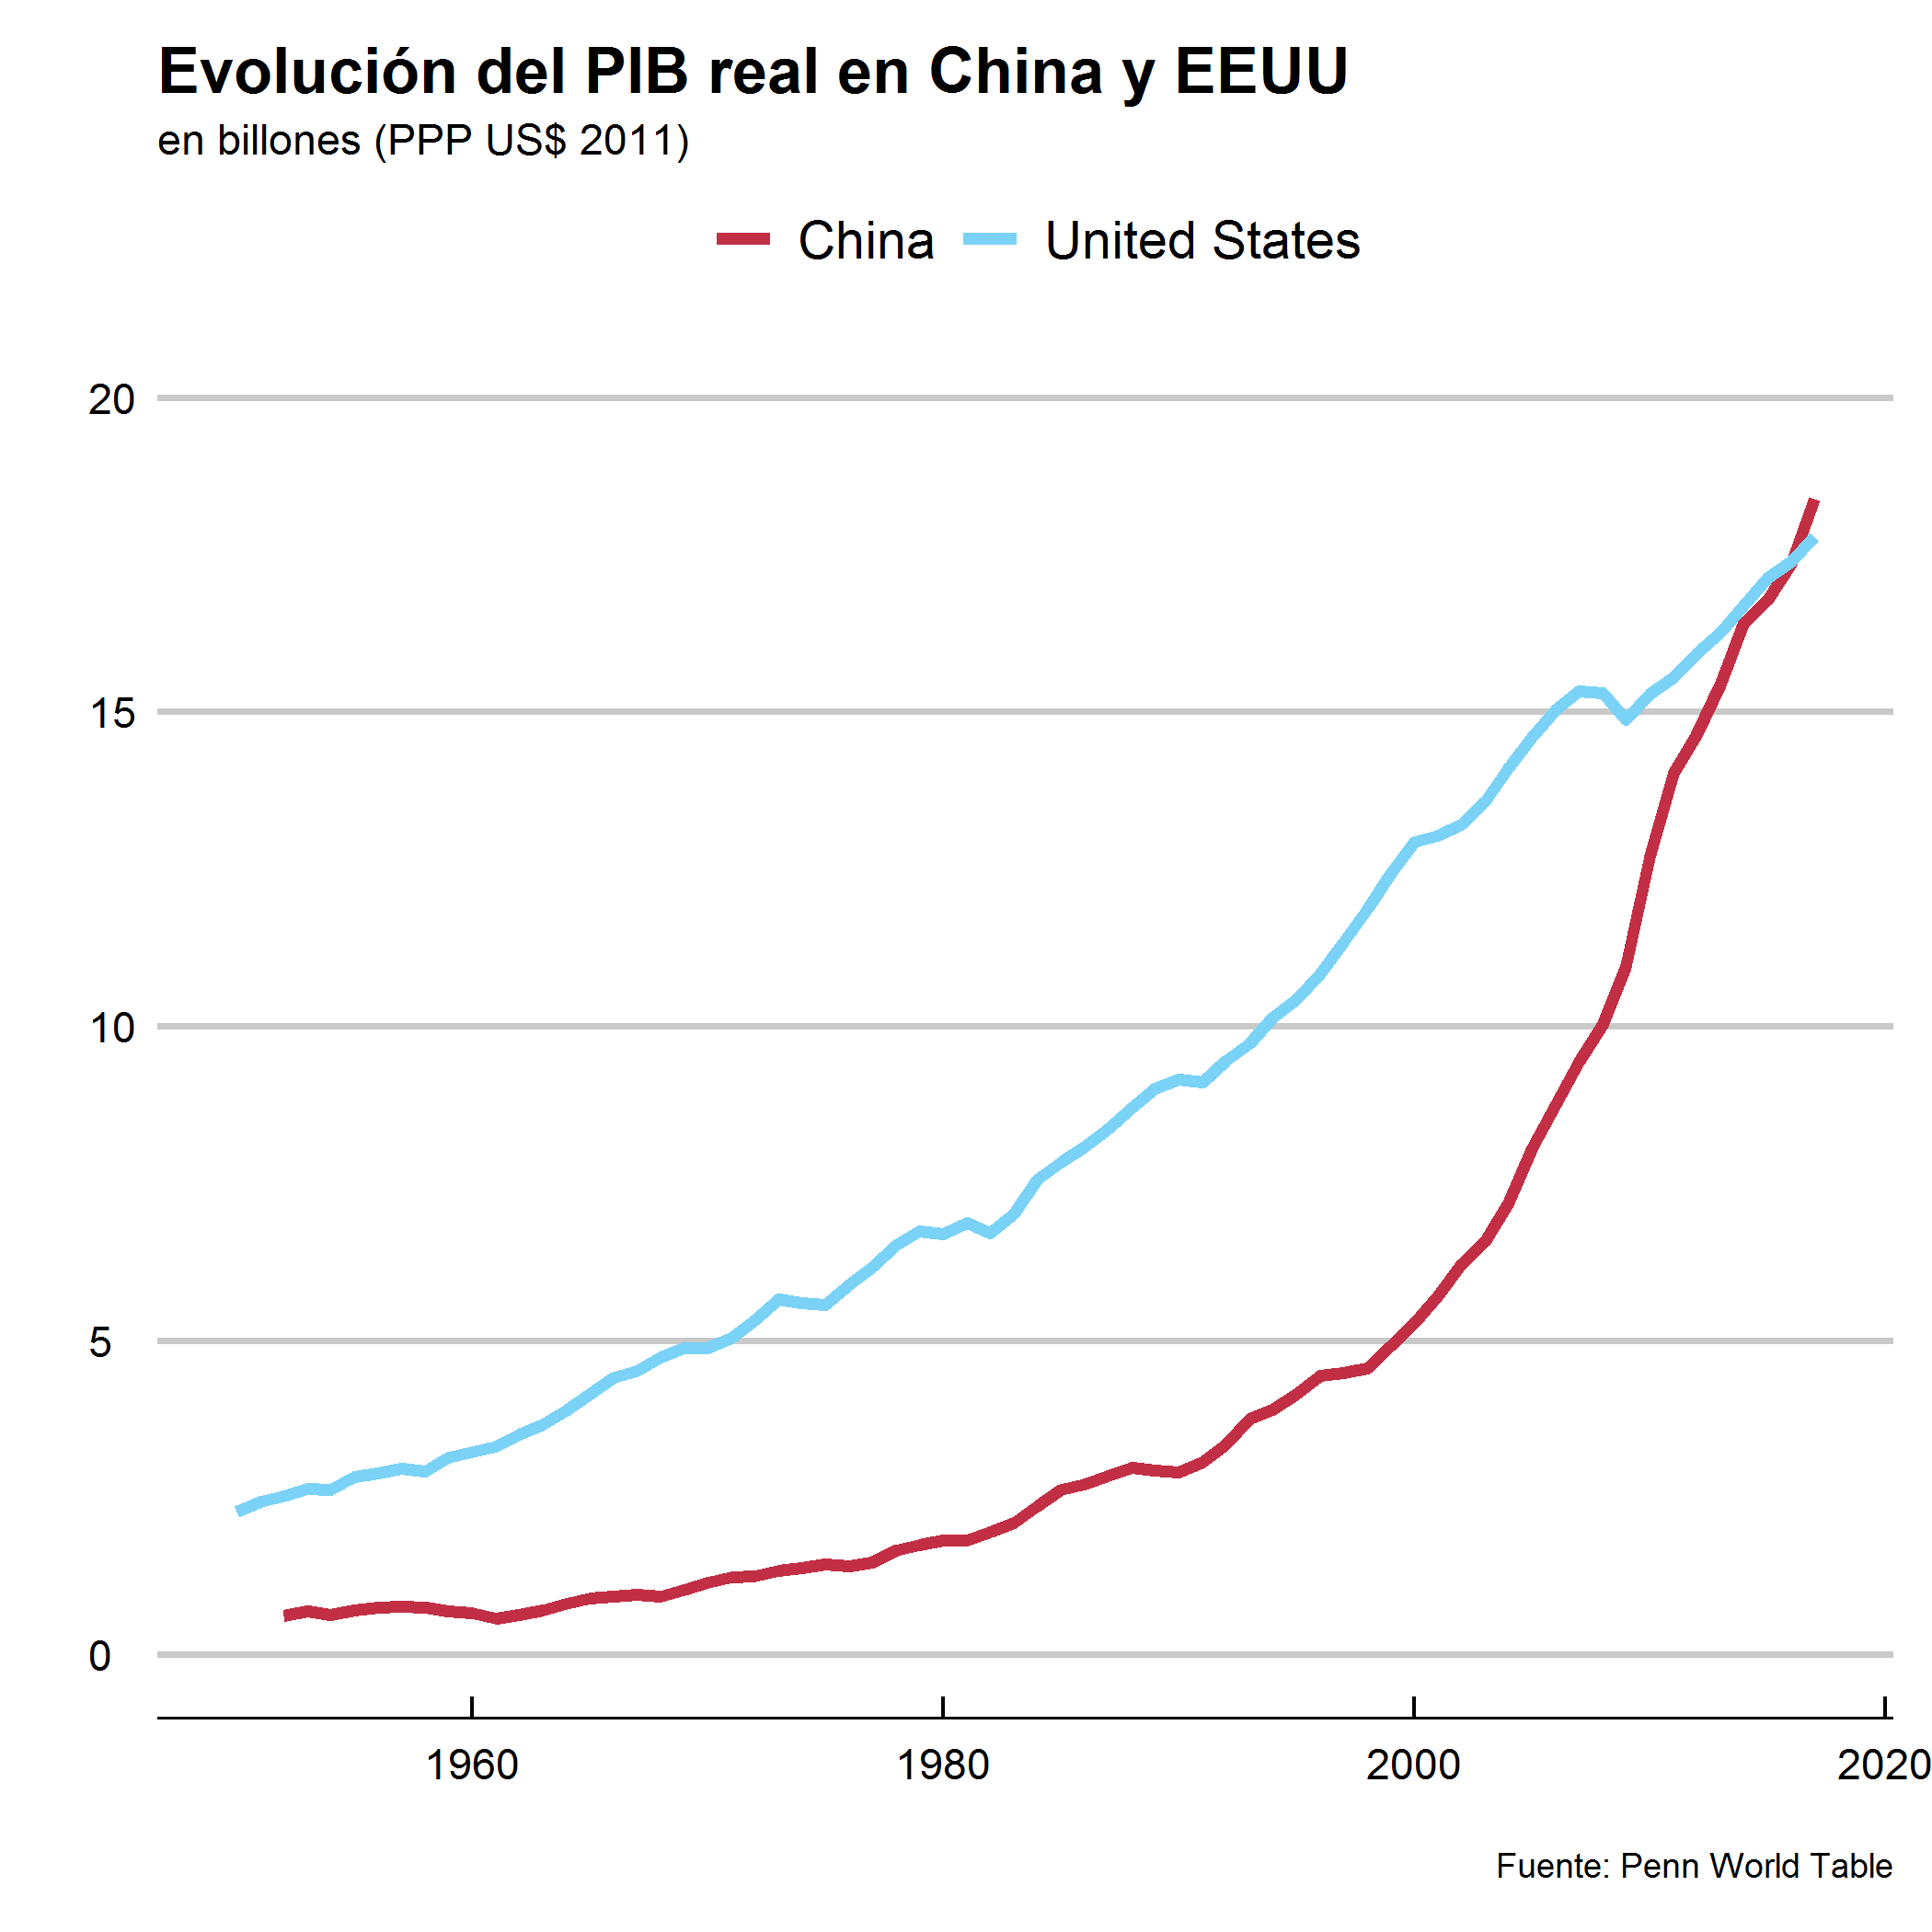
\includegraphics[width=.7\linewidth, keepaspectratio]{pib_real}
		\end{figure}
	\end{frame}

	\begin{frame}{Creciendo como China I}
		\begin{figure}
			\centering
			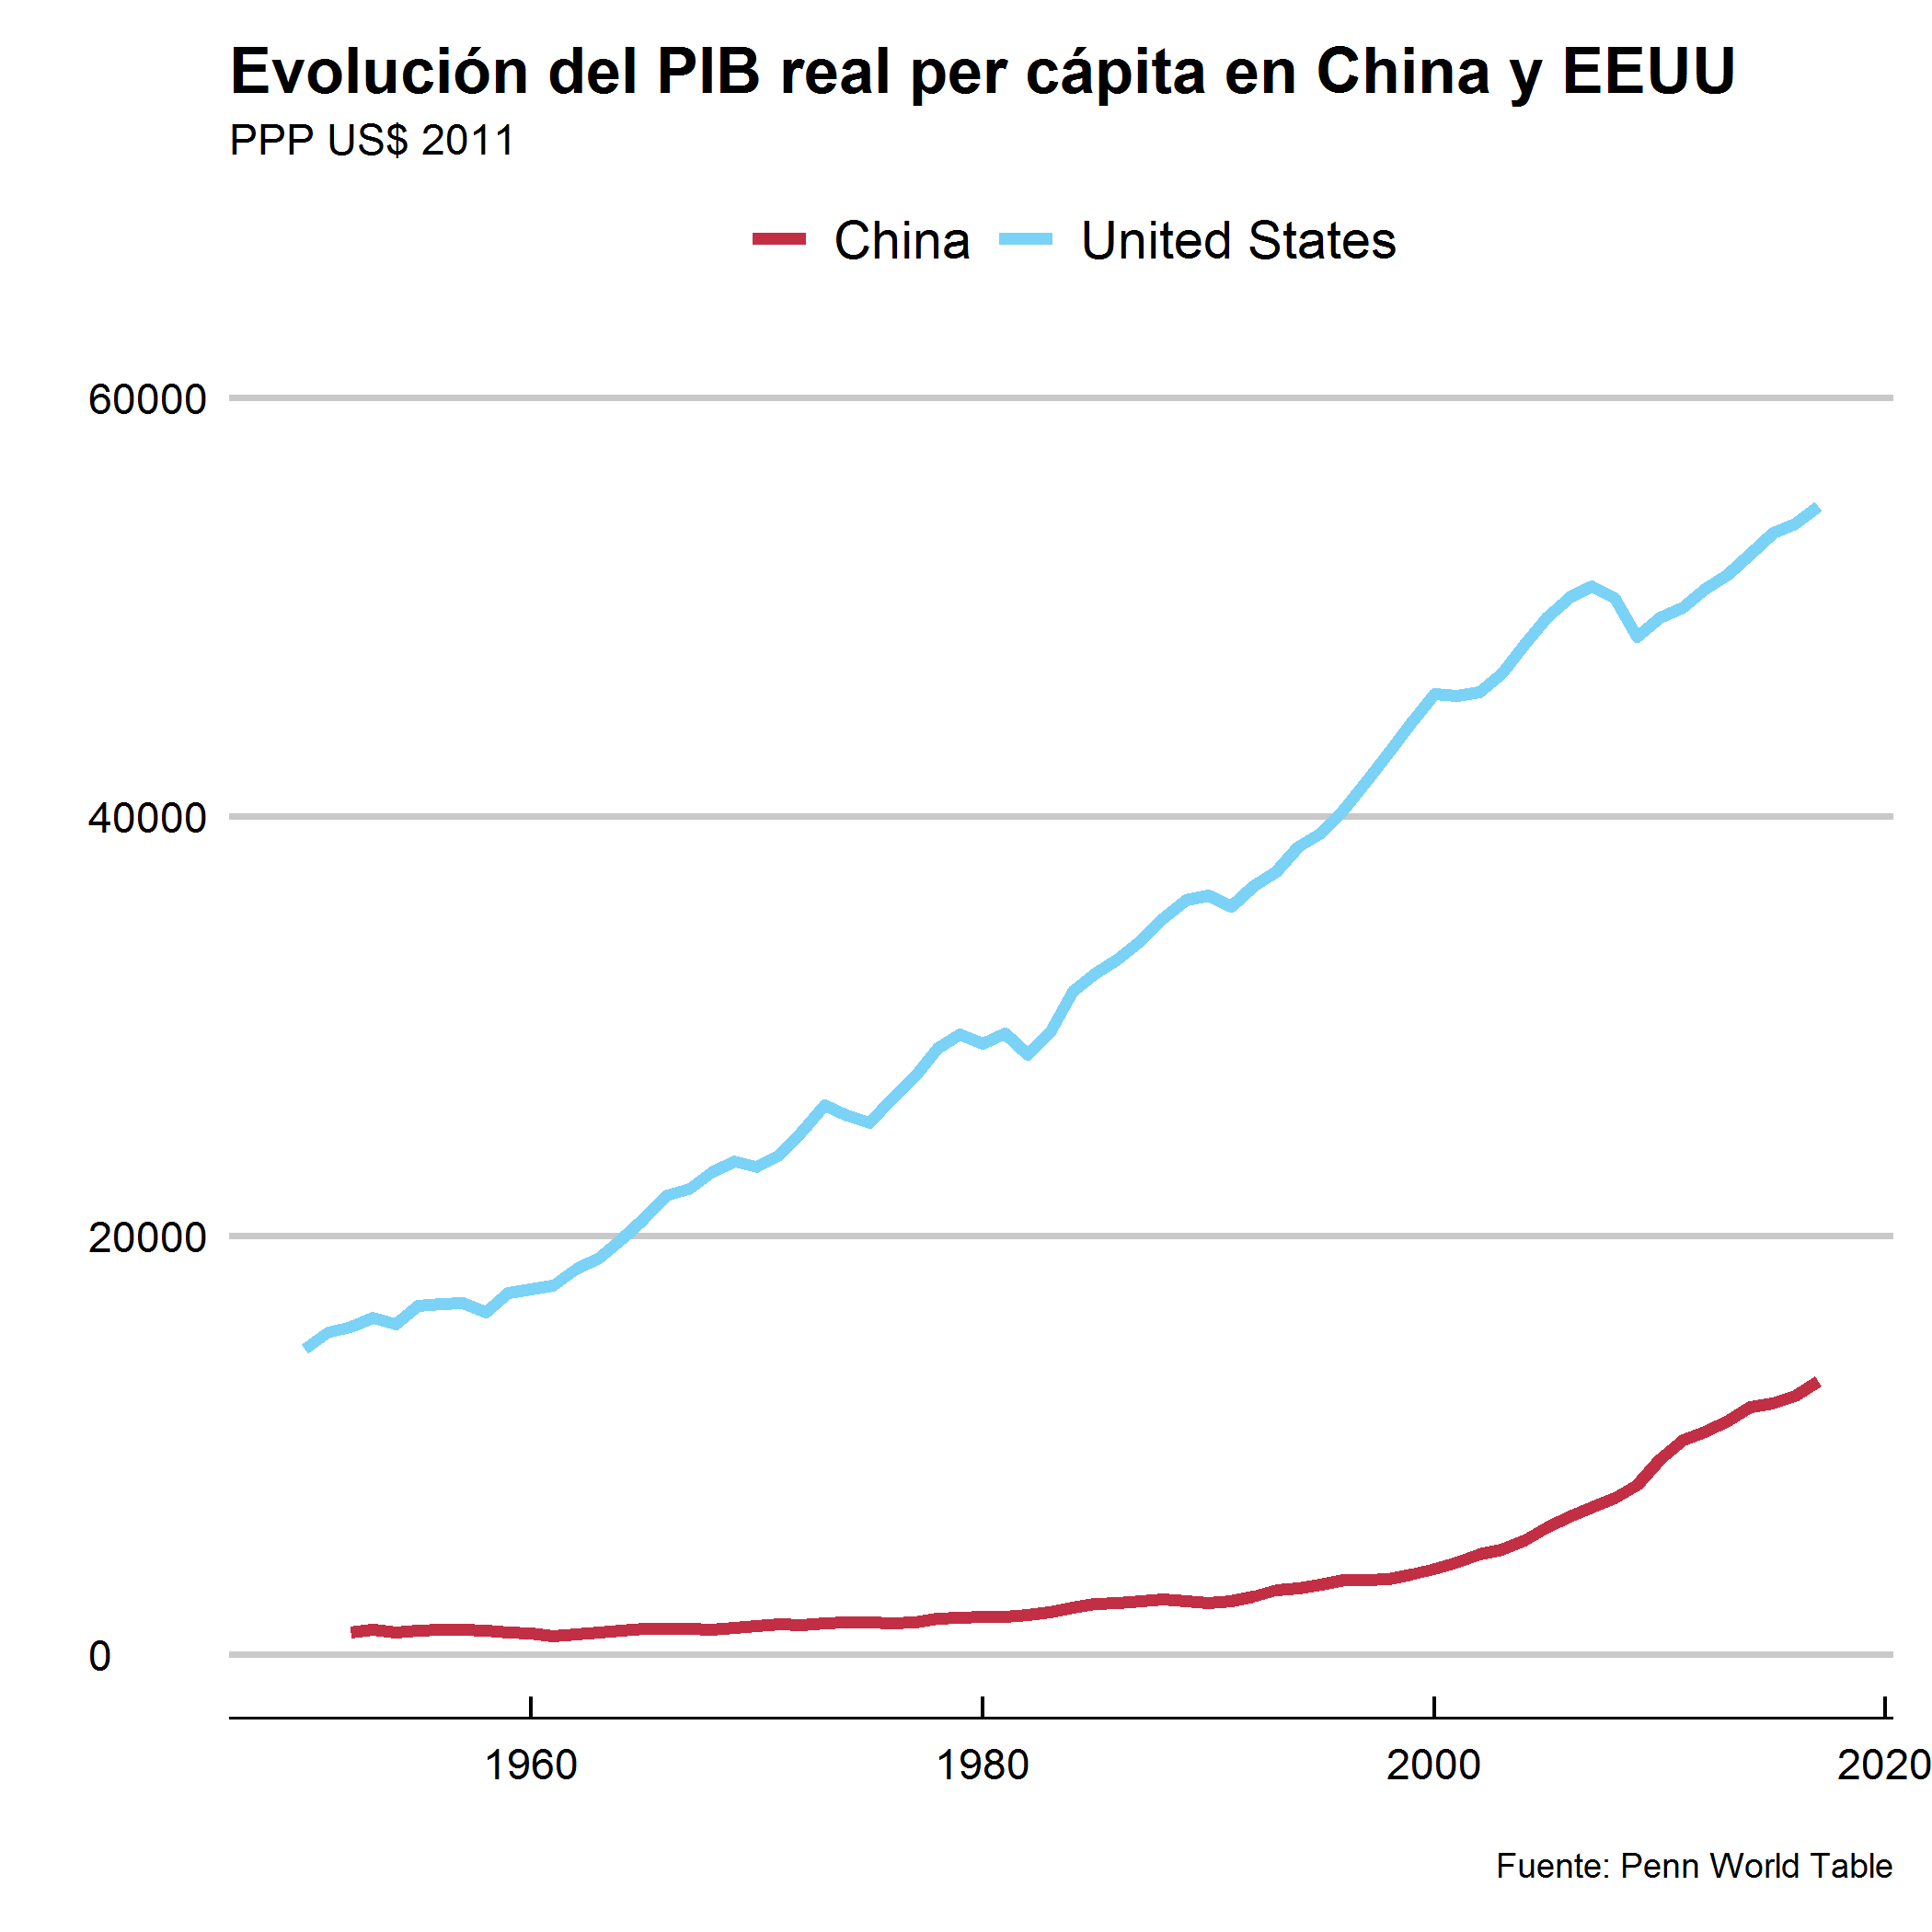
\includegraphics[width=.7\linewidth, keepaspectratio]{pib_real_pc}
		\end{figure}
	\end{frame}

	\begin{frame}{Creciendo como China II}
		\textbf{Transición hacia una economía capitalista} \\~\\
		\begin{itemize}
			\item Hasta fines de los '70 $\rightarrow$ sistema económico de planificación central
			\item Durante los '80 comienza un proceso de reforma hacia un sistema capitalista
			\item 14vo Congreso del Partido Comunista (1992) $\rightarrow$ ``economía de mercado socialista"
			\item La meta era crean un sistema de mercado como el de los países de altos ingresos con una sustancial participación del Estado en la \textbf{propiedad} de las \textbf{empresas} industriales y de servicios y un rol protagónico en la determinación de la \textbf{política económica} (Perkins, 2019).
		\end{itemize}
	\end{frame}

	\begin{frame}[c]{Creciendo como China III}
		\textbf{¿Qué explica el crecimiento sostenido de China en las últimas décadas?}
	\end{frame}

	\begin{frame}[plain]
		\centering
		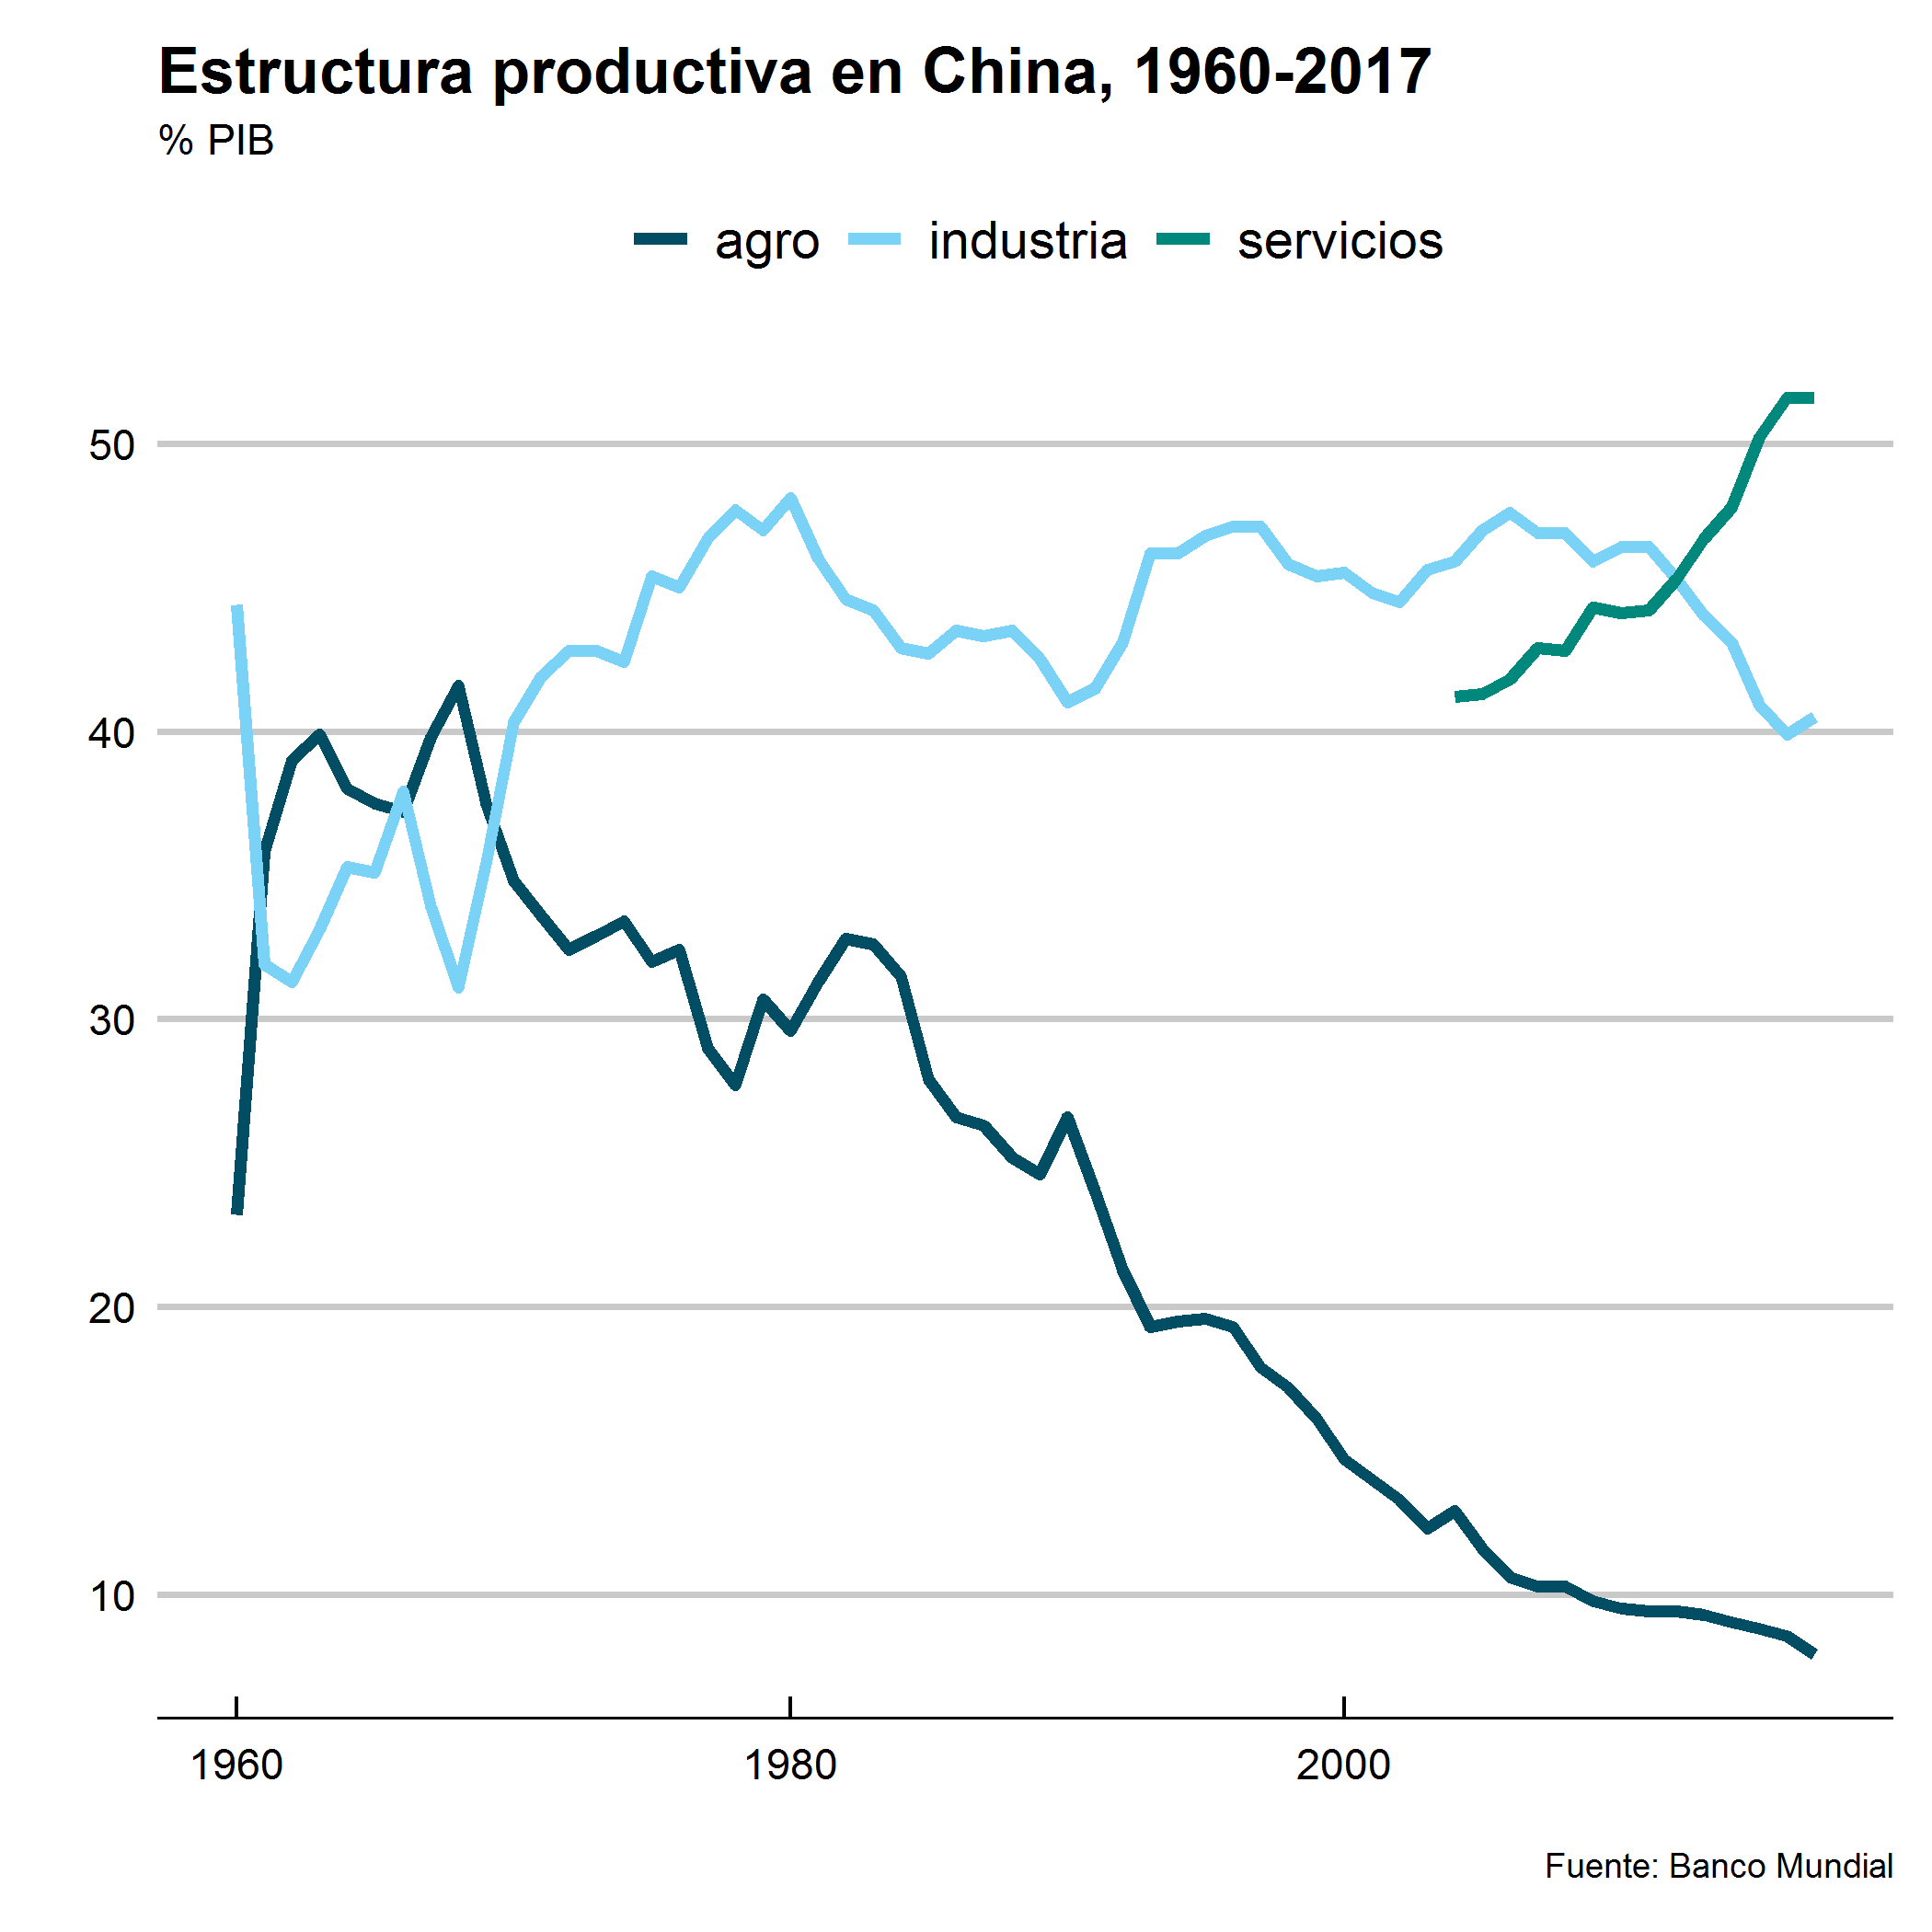
\includegraphics[width=.8\linewidth, keepaspectratio]{estr_prod_60}
	\end{frame}

	\begin{frame}[plain]
		\centering
		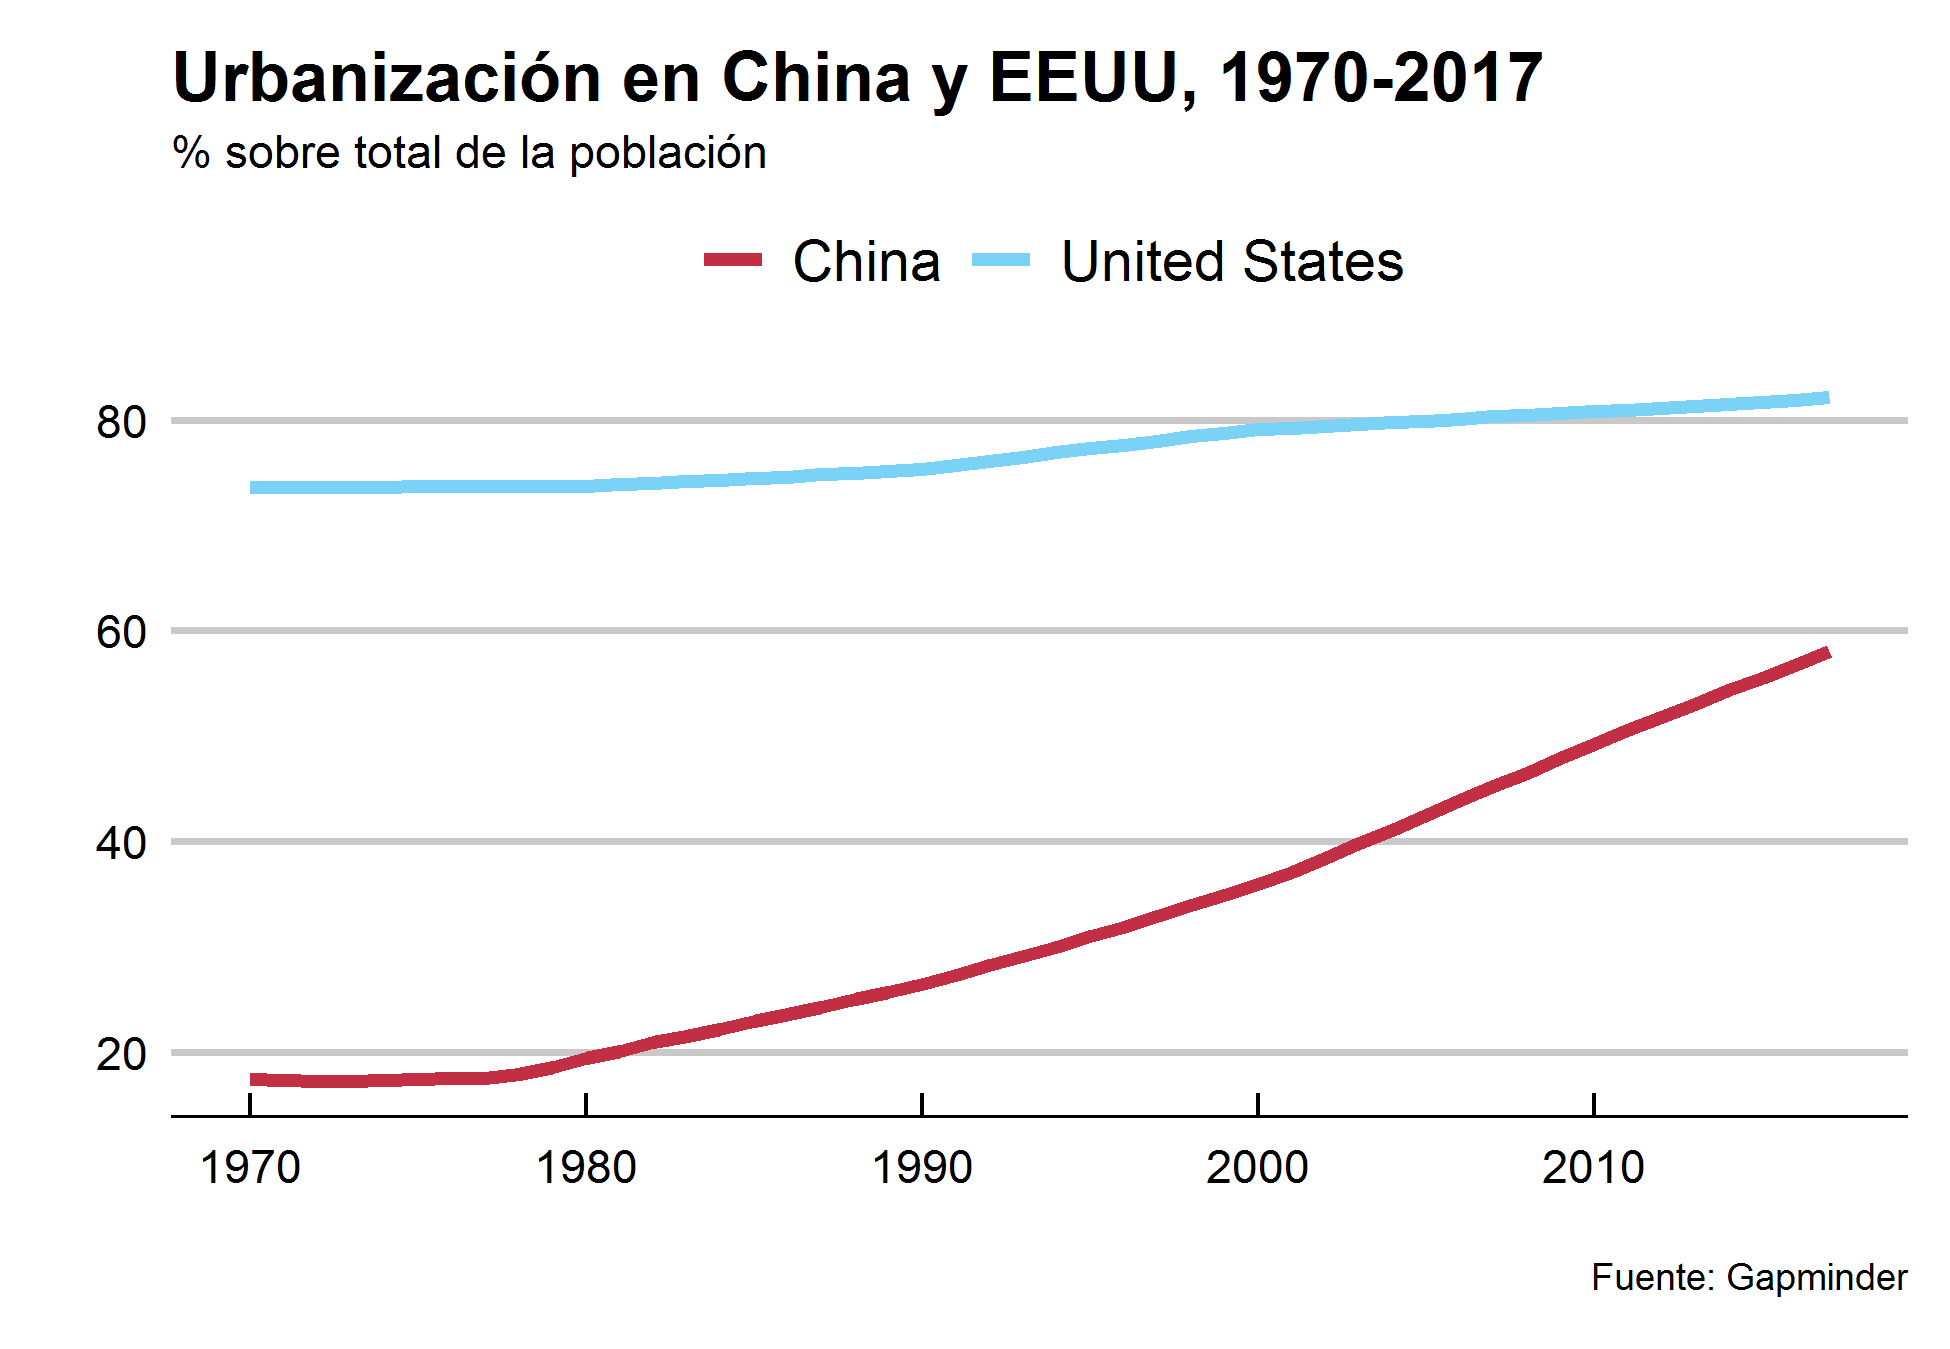
\includegraphics[width=.8\linewidth, keepaspectratio]{urban_70}
	\end{frame}

	\begin{frame}[plain]
		\begin{figure}
			\centering
			\begin{minipage}{.5\textwidth}
				\centering
				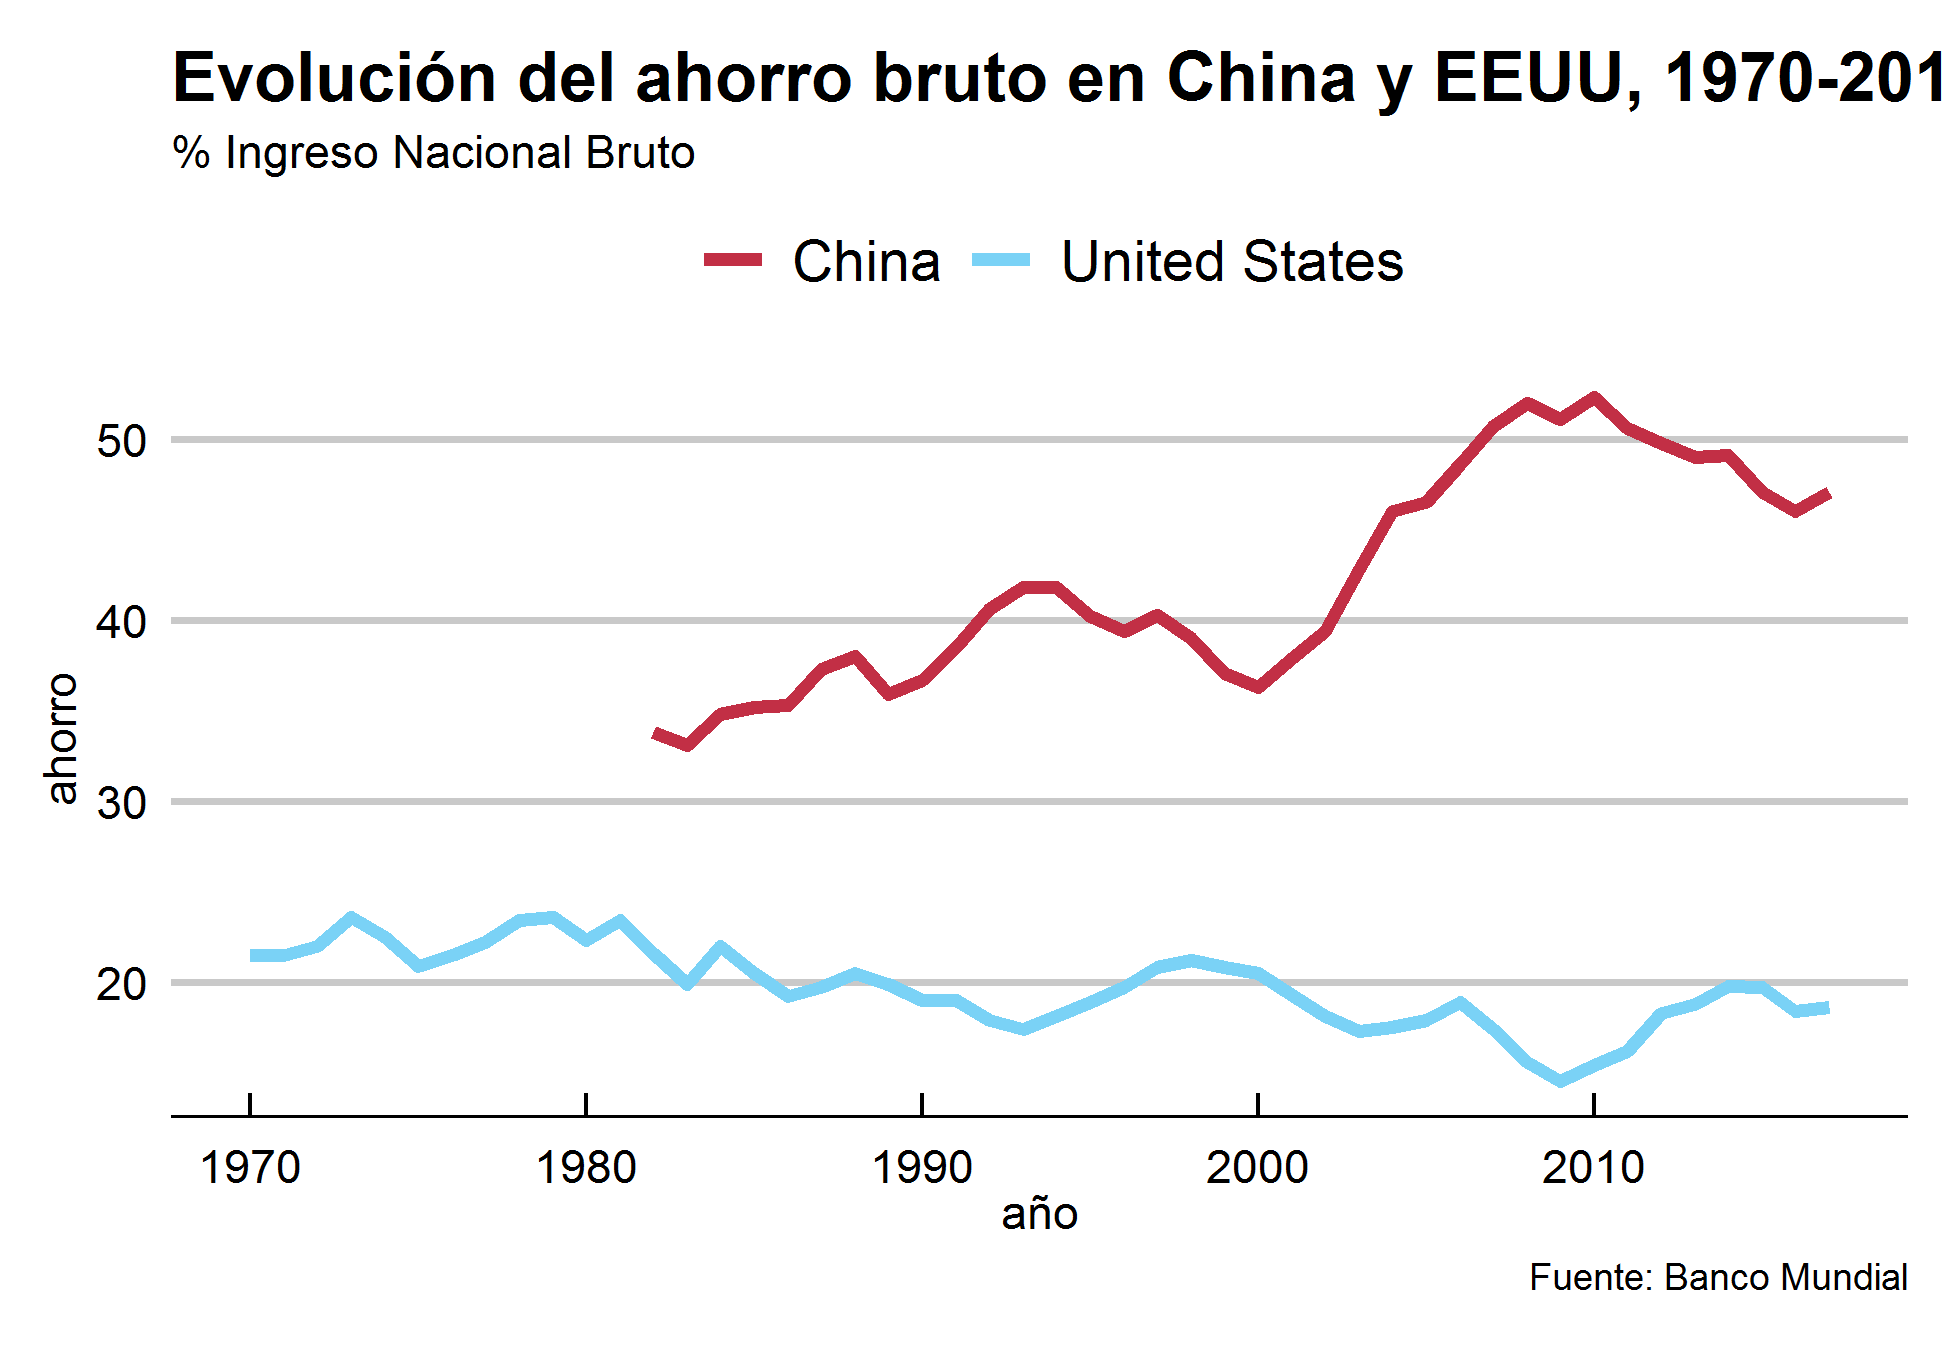
\includegraphics[width=.9\linewidth, keepaspectratio]{ahorro_70}
			\end{minipage}%
			\begin{minipage}{.5\textwidth}
				\centering
				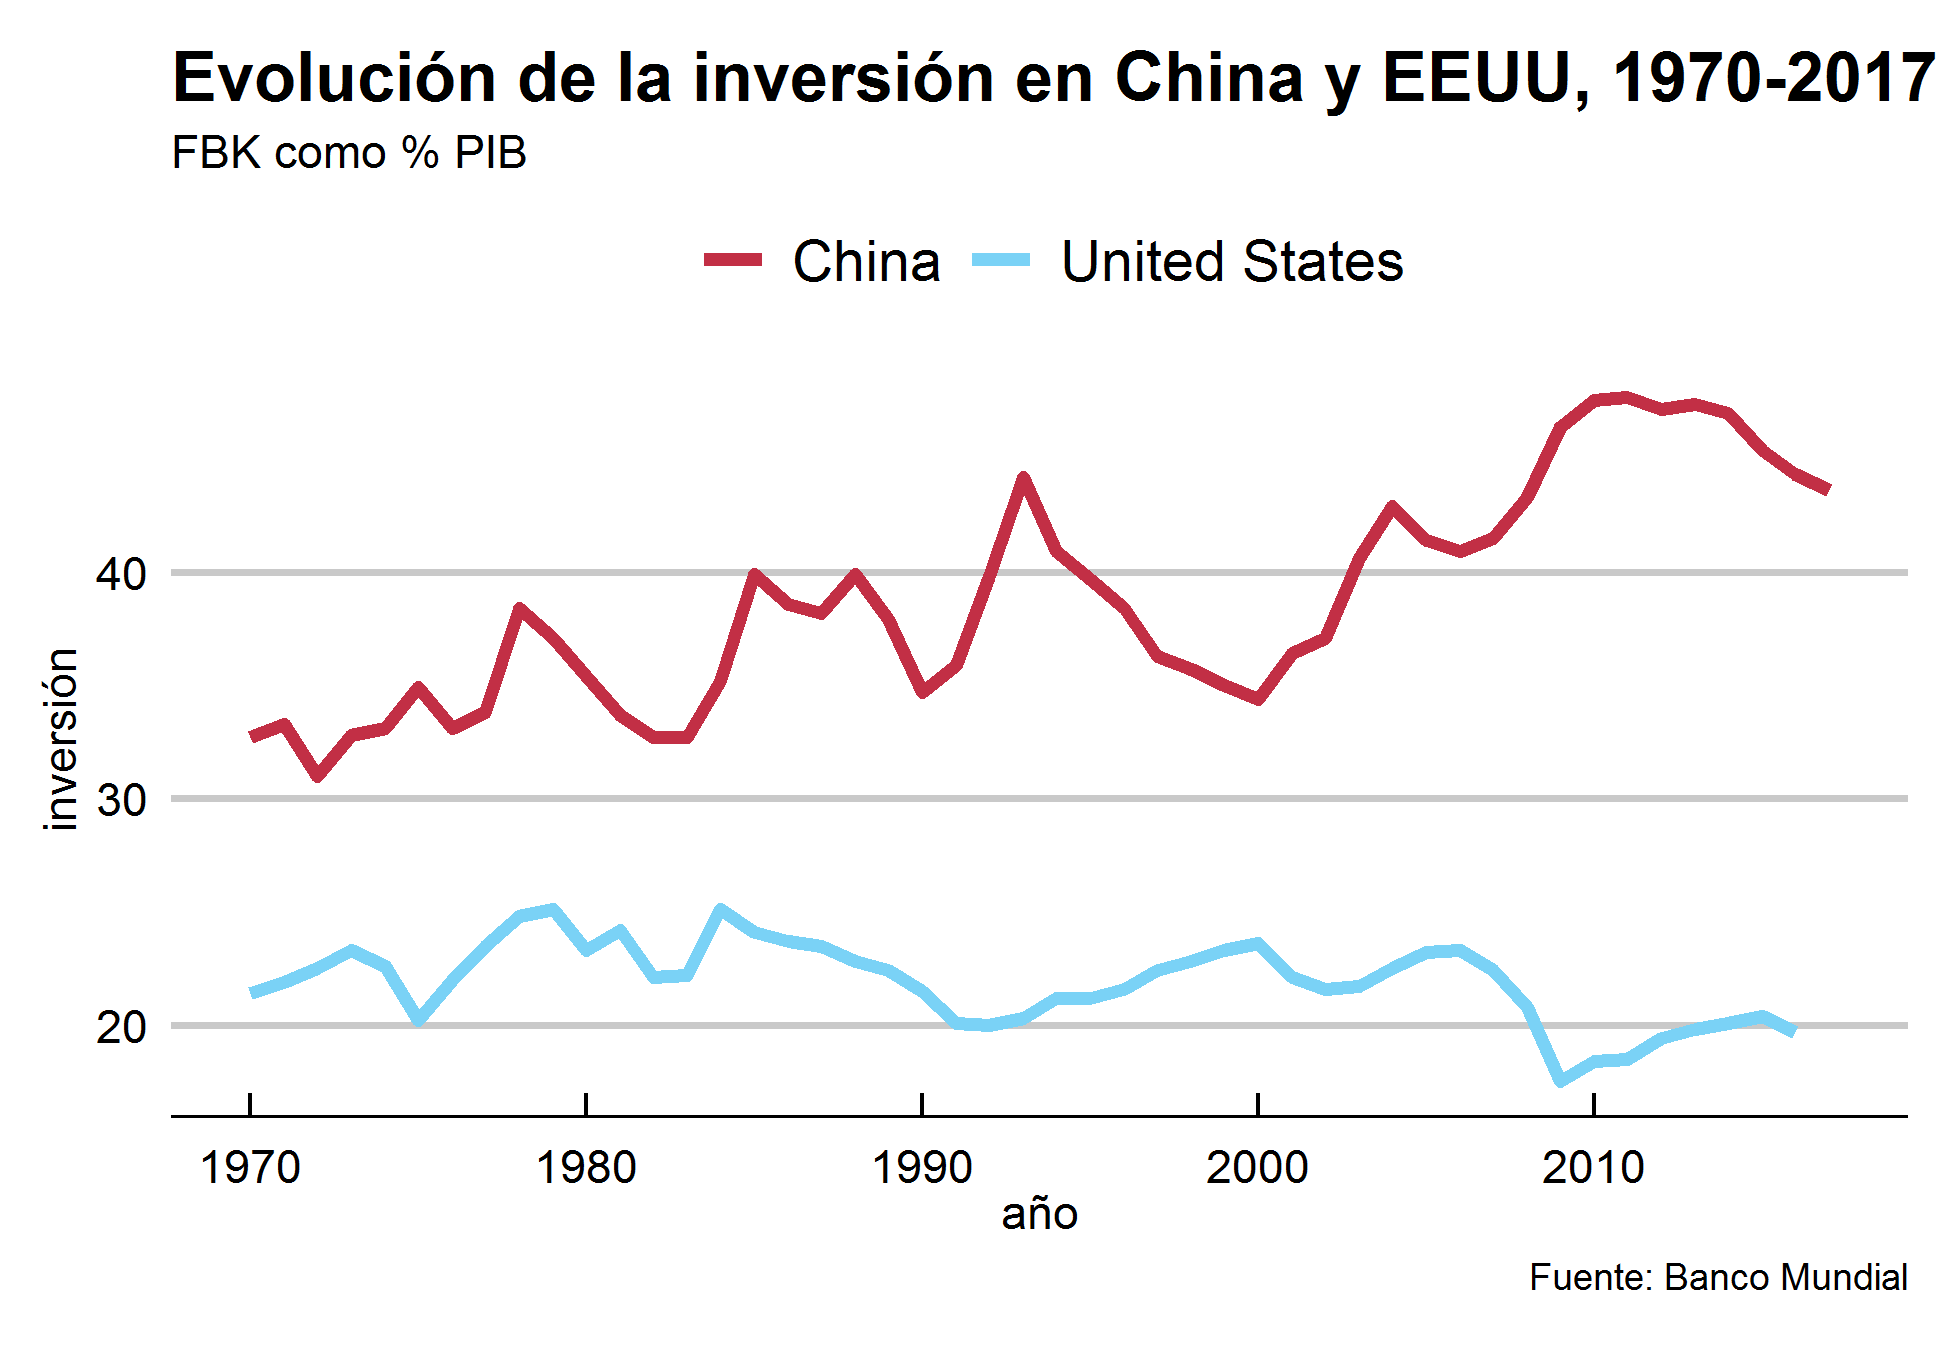
\includegraphics[width=.9\linewidth, keepaspectratio]{inversion_70}
			\end{minipage}
		\end{figure}
	\end{frame}

	\begin{frame}[plain]
		\begin{figure}
			\centering
			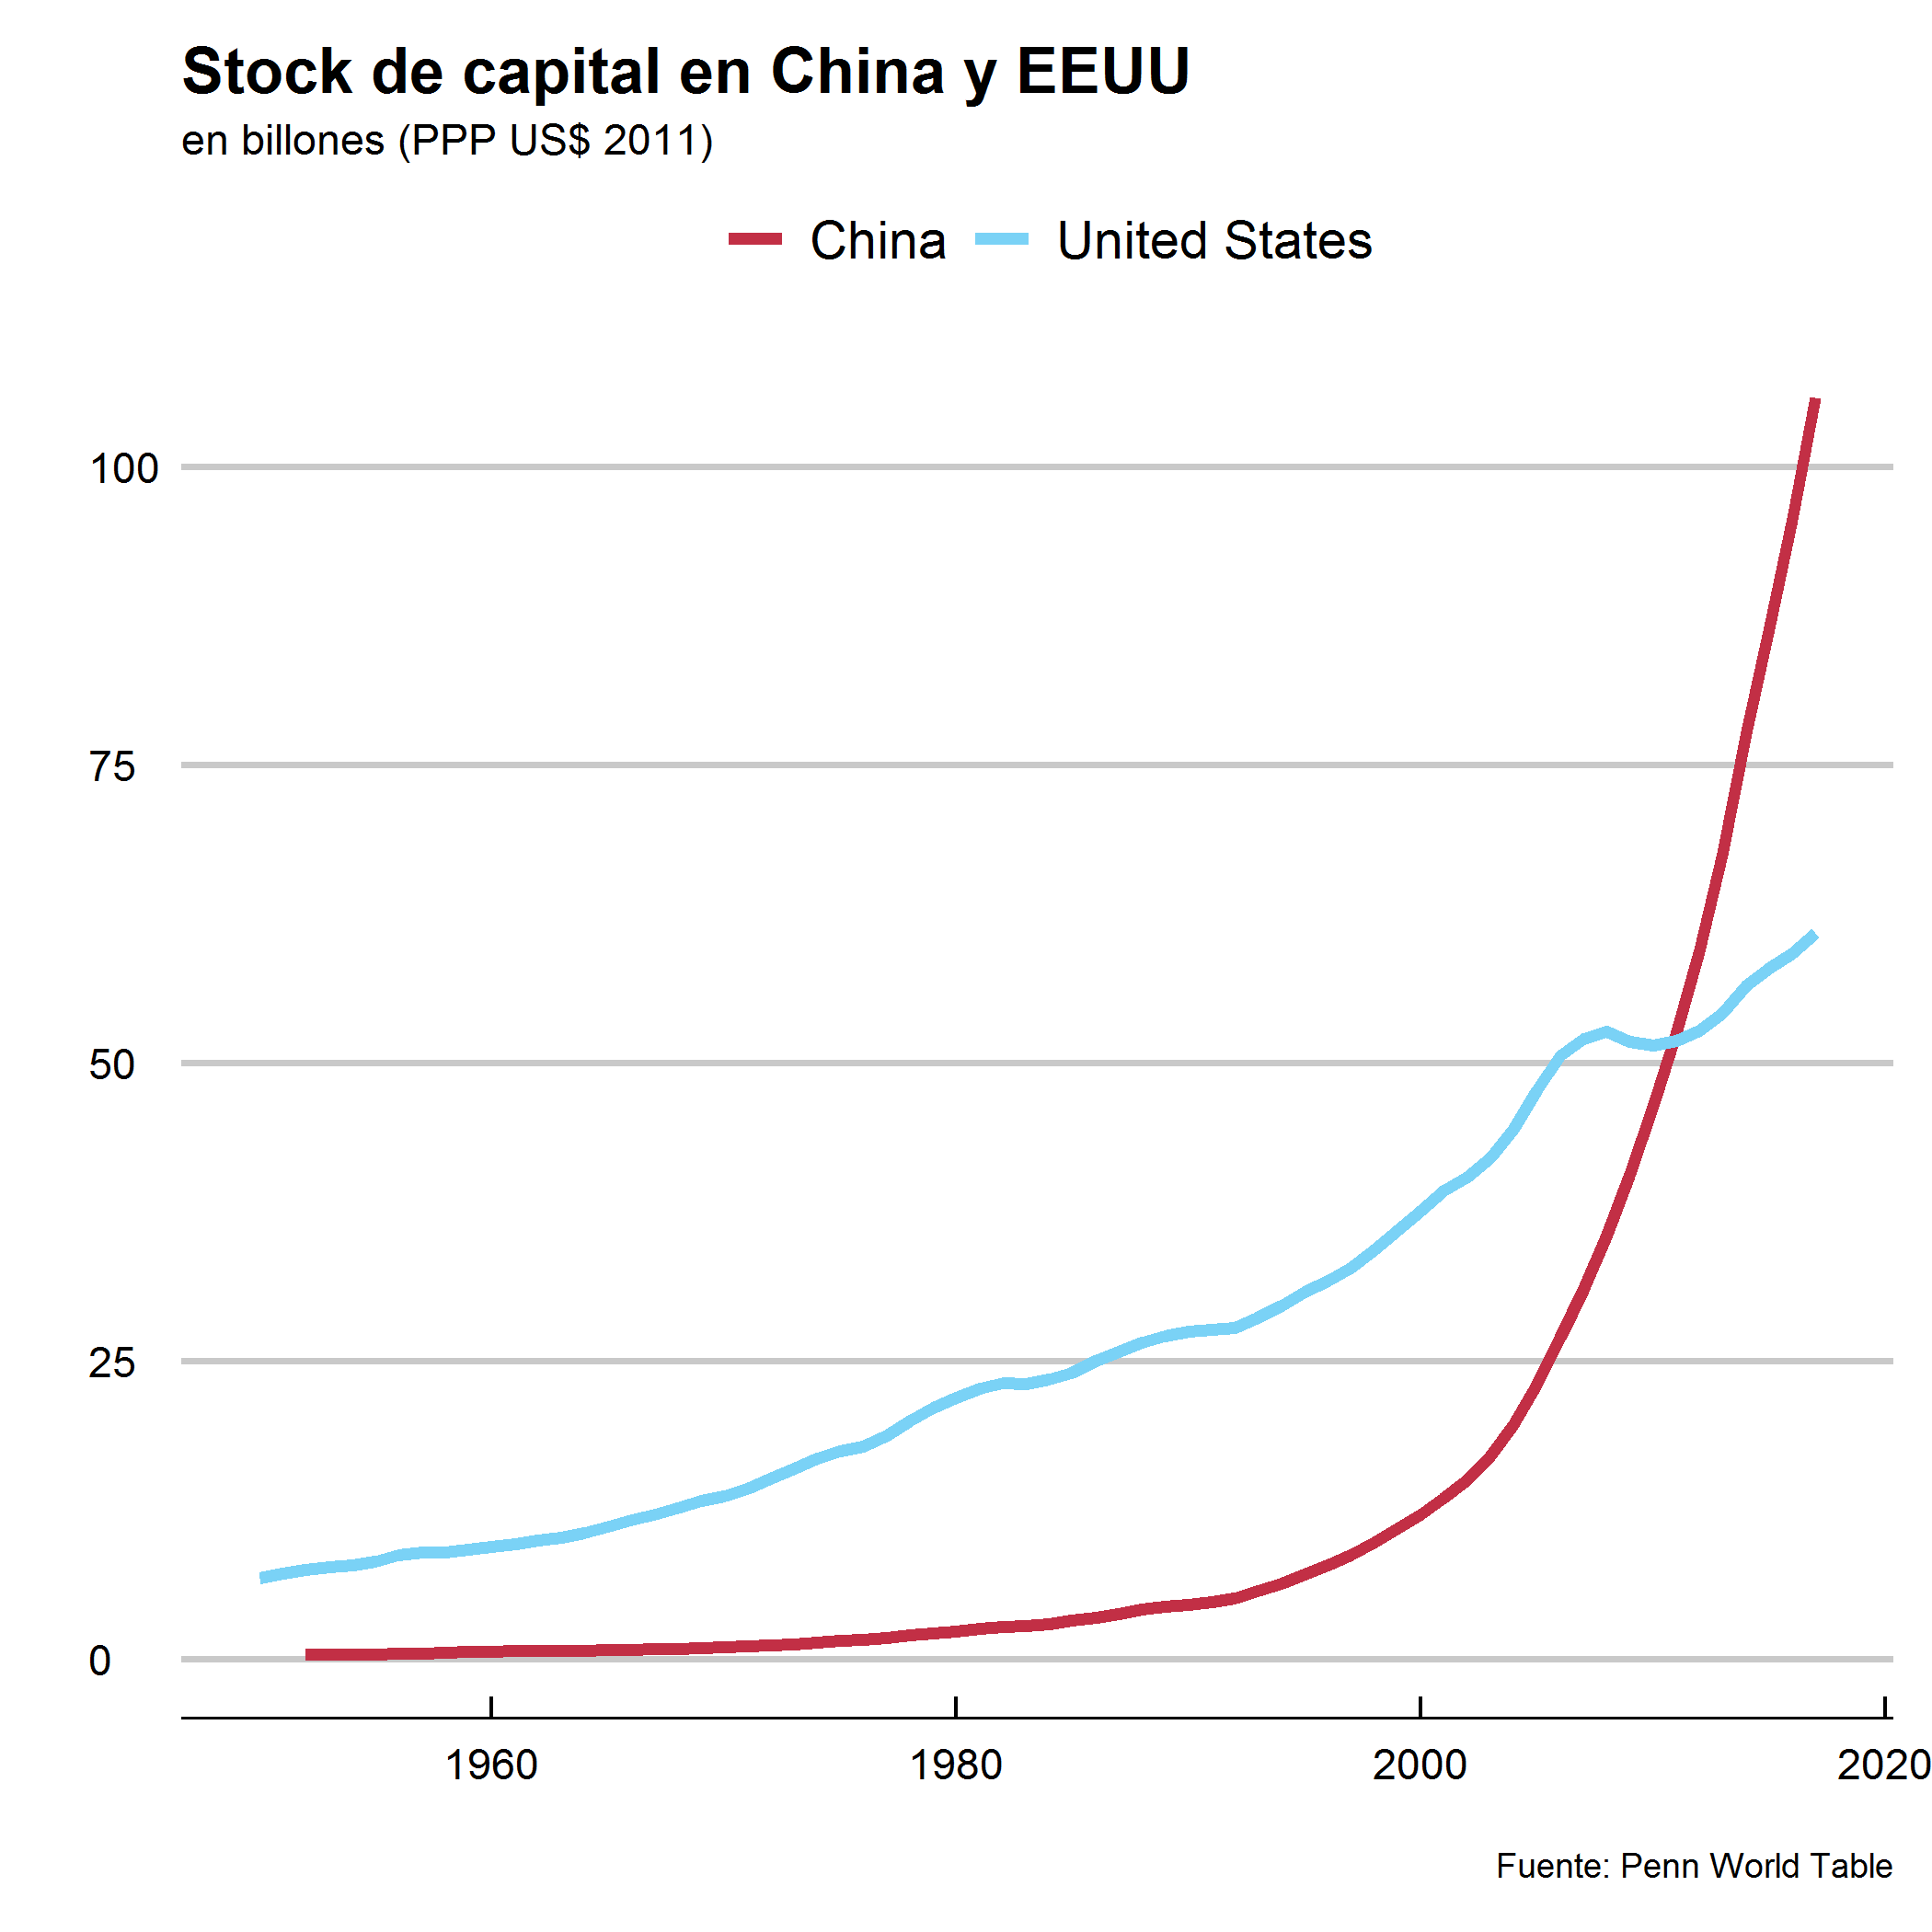
\includegraphics[width=.8\linewidth, keepaspectratio]{capital}
		\end{figure}
	\end{frame}	

	\begin{frame}[plain]
		\centering
		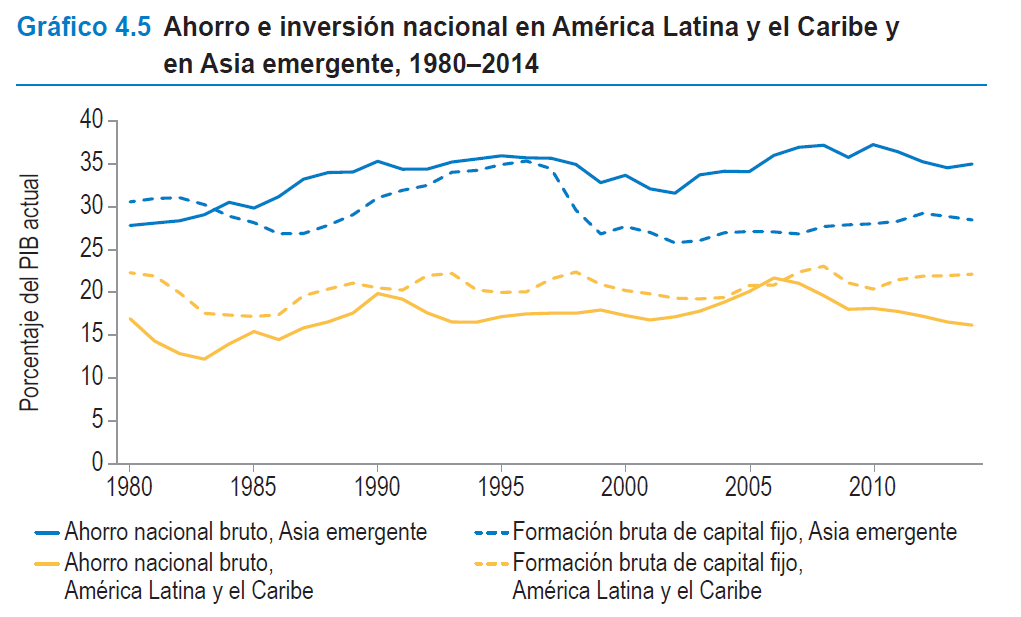
\includegraphics[width=.8\linewidth, keepaspectratio]{latam} \\
		{\footnotesize{Fuente: BID (2016), Ahorrar para desarrollarse}}
	\end{frame}

	\begin{frame}[plain]
		\begin{figure}
			\centering
			\begin{minipage}{.5\textwidth}
				\centering
				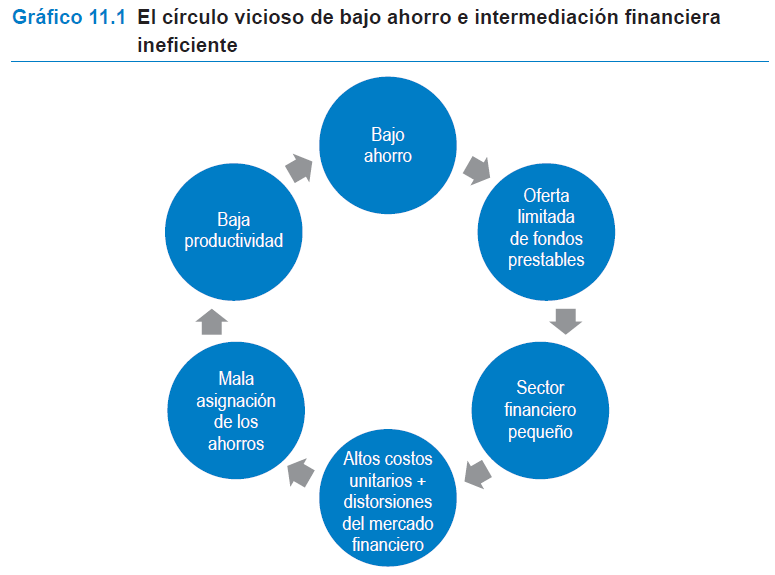
\includegraphics[width=.9\linewidth, keepaspectratio]{vicioso}
			\end{minipage}%
			\begin{minipage}{.5\textwidth}
				\centering
				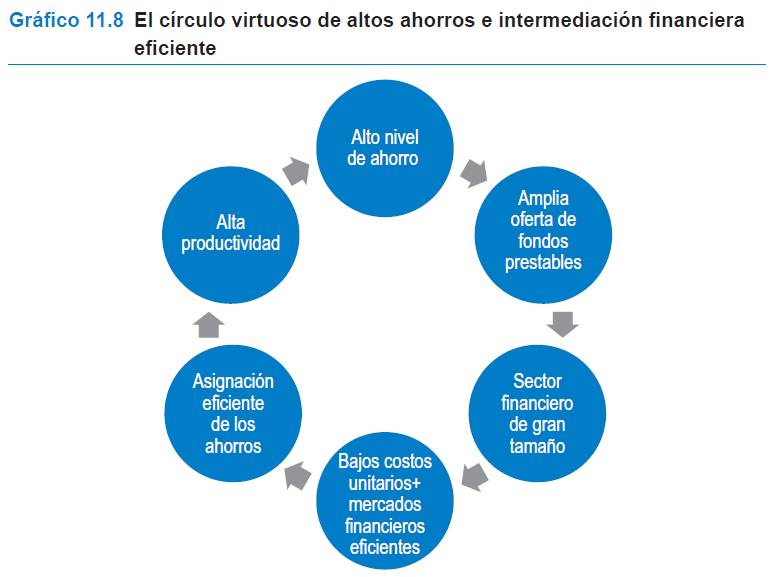
\includegraphics[width=.9\linewidth, keepaspectratio]{virtuoso}
			\end{minipage} \\~\\~\\~\\
		{\footnotesize{Fuente: BID (2016), Ahorrar para desarrollarse}}
		\end{figure}
	\end{frame}

	\begin{frame}[plain]
		\begin{figure}
			\centering
			\begin{minipage}{.5\textwidth}
				\centering
				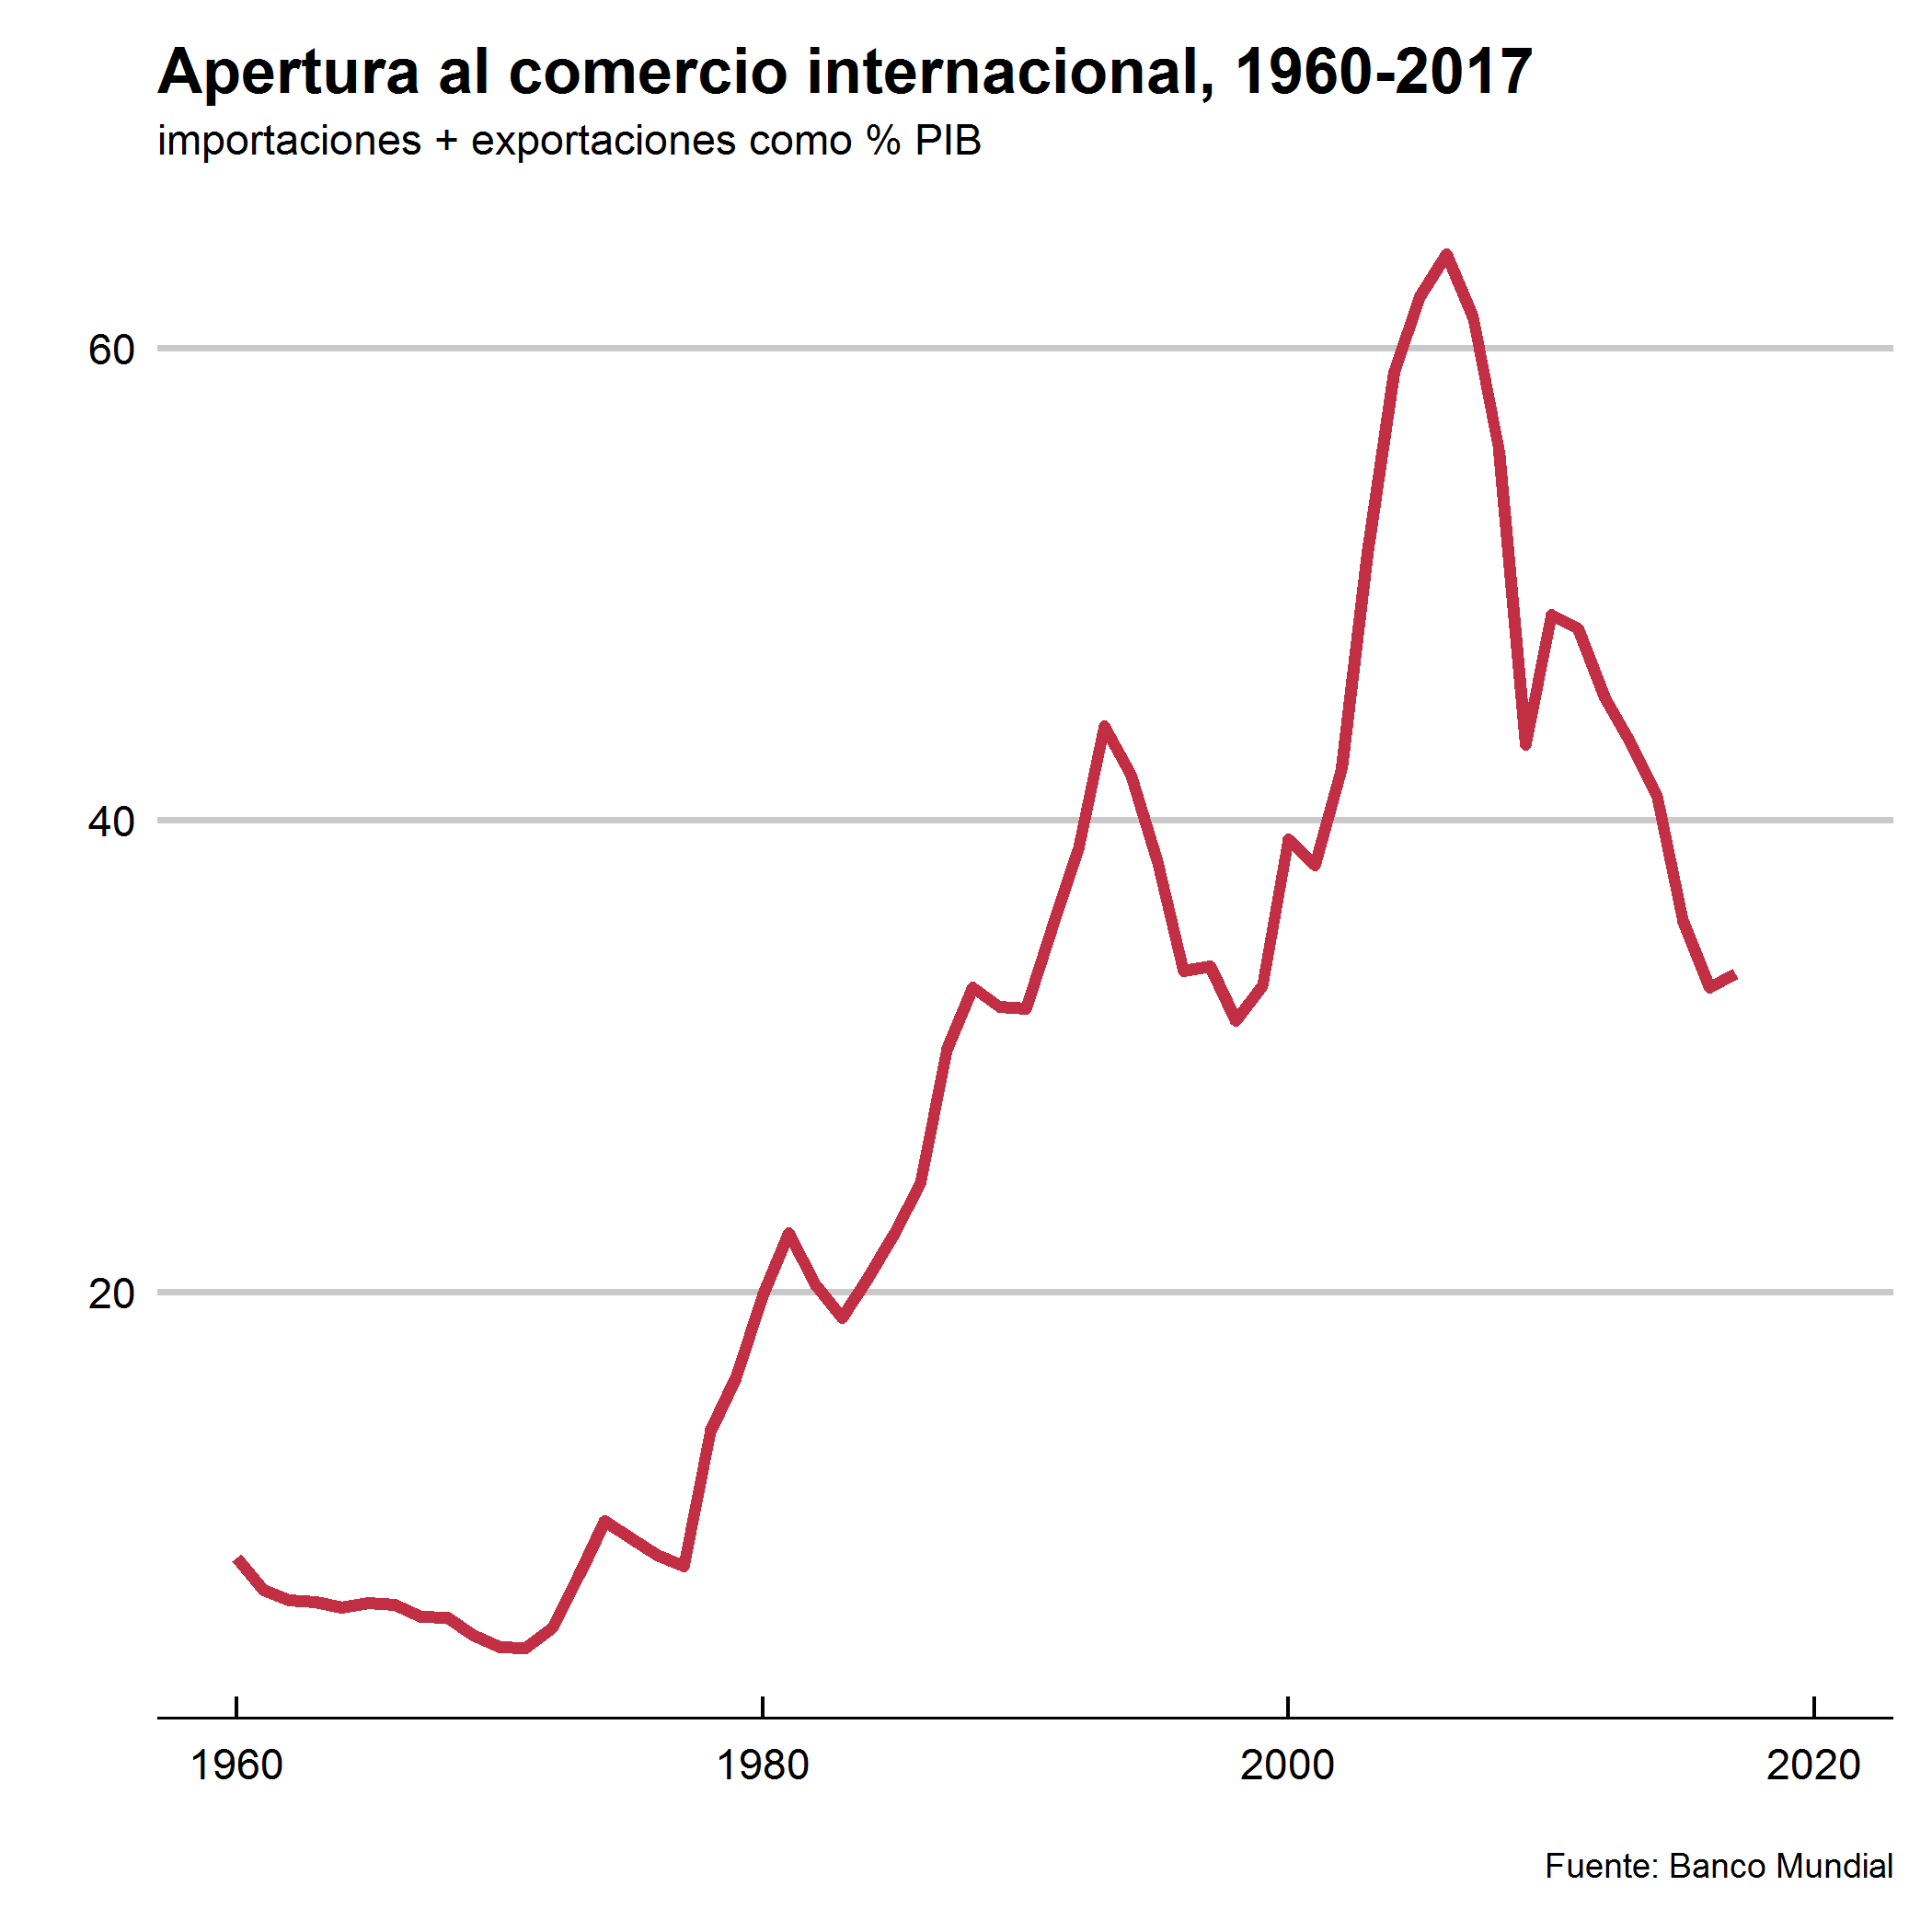
\includegraphics[width=.9\linewidth, keepaspectratio]{export_60}
			\end{minipage}%
			\begin{minipage}{.5\textwidth}
				\centering
				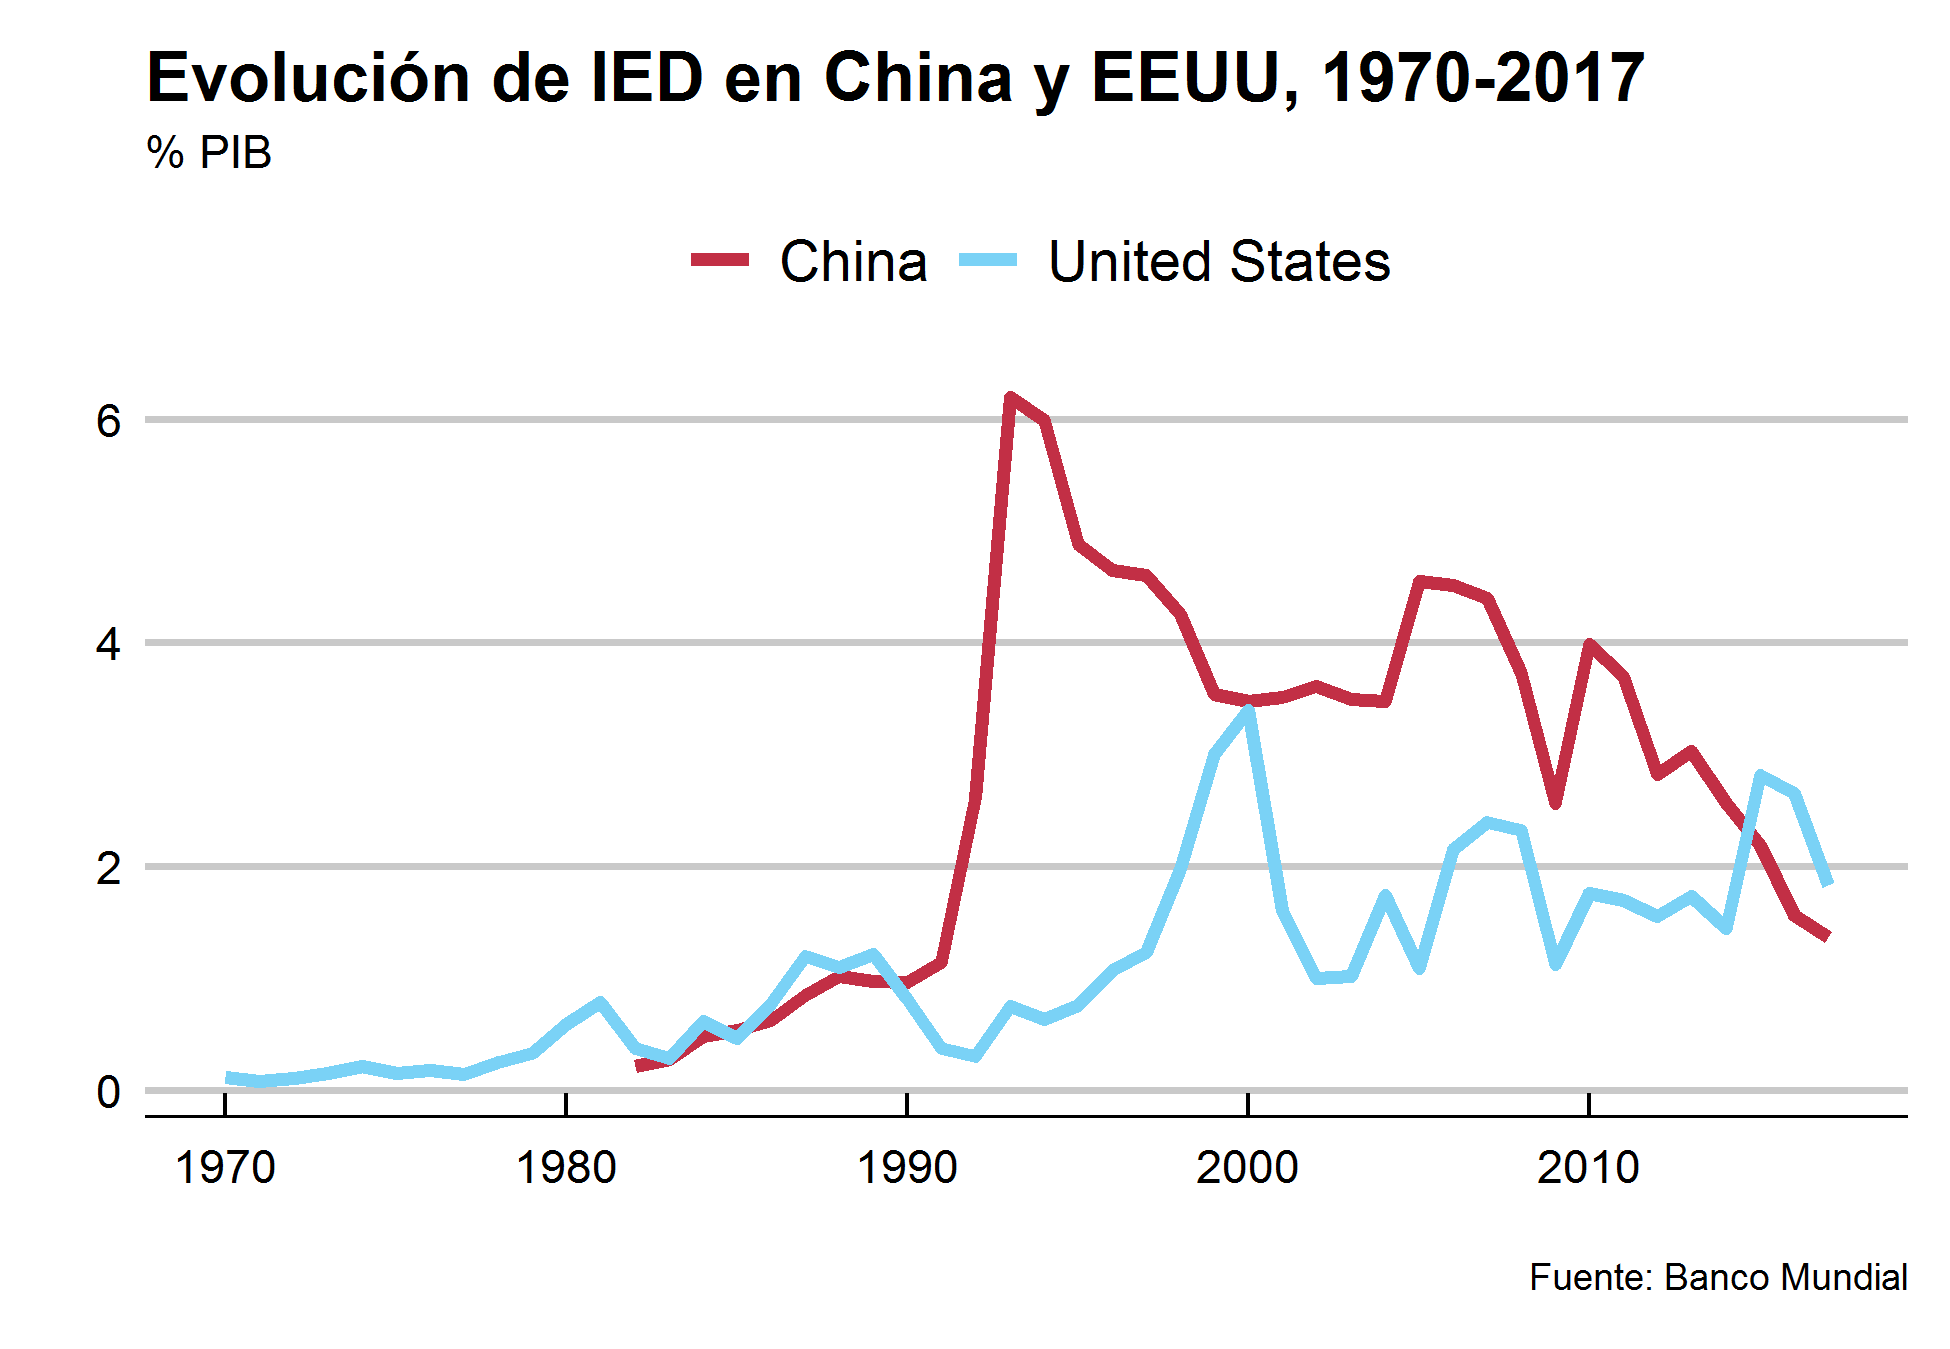
\includegraphics[width=.9\linewidth, keepaspectratio]{ied_70}
			\end{minipage}
		\end{figure}
	\end{frame}

	\begin{frame}[plain]
		\textbf{Participación de China en el valor agregado y exportaciones en manufacturas a nivel mundial:}
		\medskip
		\begin{figure}
			\centering
			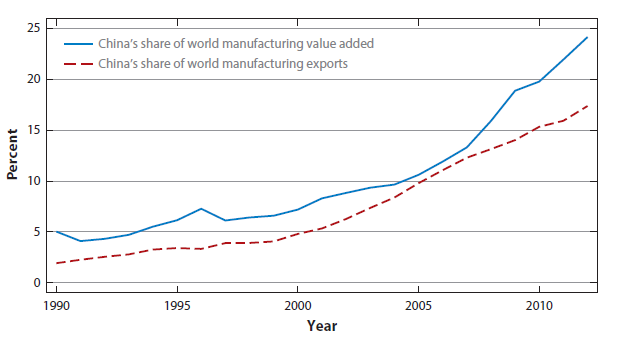
\includegraphics[width=.7\linewidth, keepaspectratio]{manufacturing} \\
			{\footnotesize{Fuente: Autor et al. (2016). The china shock: Learning from labor-market adjustment to large changes in trade}}
		\end{figure}
	\end{frame}

	\begin{frame}{Creciendo como China III}
			\textbf{¿Qué explica el crecimiento sostenido de China en las últimas décadas?}\\~\\
			\pause
			\begin{itemize}
				\item Transformación hacia economía capitalista con fuerte participación del Estado (\textbf{estado desarrollista})
				\begin{itemize}
					\item Se permite la competencia en ciertos mercados
					\item Surgen empresas privadas
					\item Regulaciones y leyes que protegen la propiedad privada
				\end{itemize}
				\item Reasignación de los trabajadores desde el sector agrícola hacia el sector industrial y de servicios $\rightarrow$ proceso de urbanización
				\item Elevadas tasas de ahorro e inversión en capital
				\item Apertura progresiva de la economía al comercio internacional promoviendo y protegiendo el desarrollo de industrias exportadoras.
			\end{itemize}
	\end{frame}

	\begin{frame}{Creciendo como China IV}
		\textbf{¿Puede ser este tipo de crecimiento sostenible?} \\~\\
		\pause
		\begin{itemize}
			\item Vimos que una de las claves de una economía dinámica es la competencia y los incentivos a innovar. ¿La propiedad de las empresas por parte del Estado garantiza esta dinámica?
		\end{itemize}
	\end{frame}

	\begin{frame}{Creciendo como China V}
		\begin{figure}
			\centering
			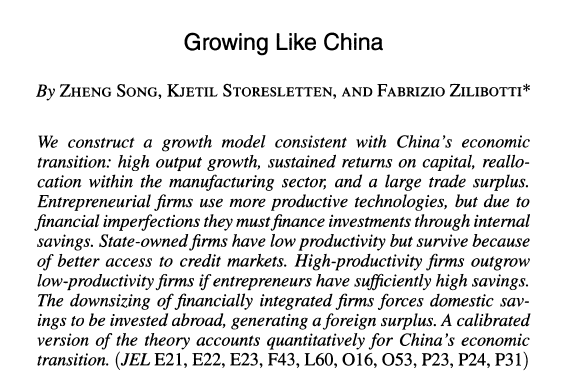
\includegraphics[width=.6\linewidth, keepaspectratio]{growing_like_china}
		\end{figure}
		\begin{itemize}
			\item Basado en estudios previos que demuestran que las empresas estatales son menos productivas, Zheng et al. (2011) encuentan que la reasignación de factores desde empresas menos productivas hacia aquellas más productivas es un motor importante del desempeño económico de China.
		\end{itemize}
	\end{frame}

	\begin{frame}{Creciendo como China VI}
		\begin{itemize}
			\item También vimos que cuando las leyes que regulan los mercados son muy rígidas o cuando la protección a la propiedad privada no es clara se generan ineficiencias.
		\end{itemize}
	\end{frame}

	\begin{frame}[plain]
		\begin{figure}
			\centering
			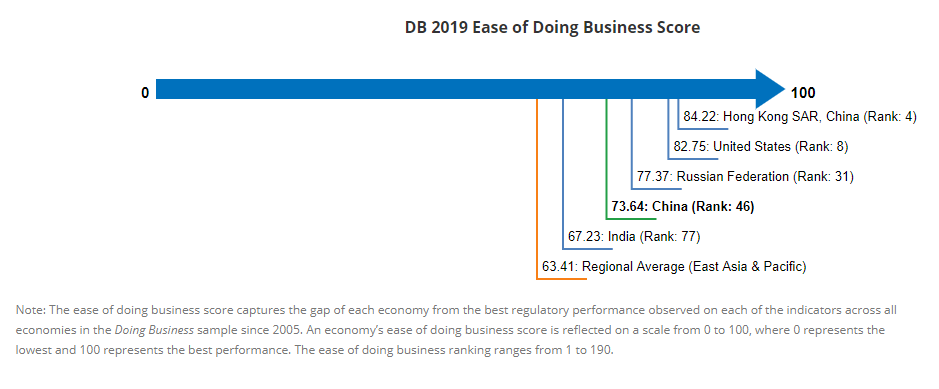
\includegraphics[width=\linewidth, keepaspectratio]{doing_business_rank} \\
			{\footnotesize{Fuente: Doing Business}}
		\end{figure}
	\end{frame}

	\begin{frame}[plain]
		\begin{figure}
			\centering
			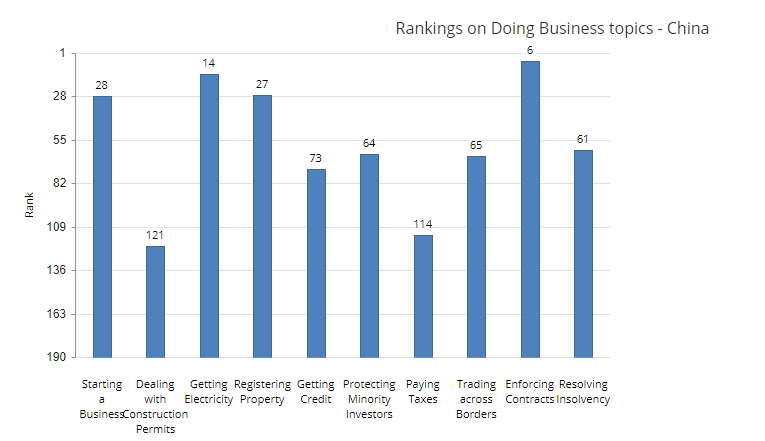
\includegraphics[width=\linewidth, keepaspectratio]{doing_business_rank_components} \\
			{\footnotesize{Fuente: Doing Business}}
		\end{figure}
	\end{frame}

	\begin{frame}{Creciendo como China VII}
		\begin{itemize}
			\item Formular una hipótesis respecto a qué explica el crecimiento sostenido de China aplicando los conceptos vistos en el curso y la evidencia.
			\item Formular posibles respuestas.
		\end{itemize}
	\end{frame}	

	\begin{frame}{Links}
		\begin{itemize}
			\item Top 20 Country GDP (PPP) History \& Projection (1800-2040):  \href{https://www.youtube.com/watch?v=4-2nqd6-ZXg}{https://www.youtube.com/watch?v=4-2nqd6-ZXg}
			\item Repositorio con los datos, material bibliográfico y código para generar los gráficos: \href{https://github.com/GabrielMerlo/DyB_actividad_1}{https://github.com/GabrielMerlo/DyB\_actividad\_1}
		\end{itemize}
	\end{frame}

\end{document}